\documentclass[tikz]{standalone}

% Packages
\usepackage[T1]{fontenc}
\usepackage{lmodern} % nicer sans serif when using \sffamily
\usepackage{tikz}
\usetikzlibrary{arrows.meta, positioning, shapes.misc, shapes.symbols, calc}

\begin{document}
	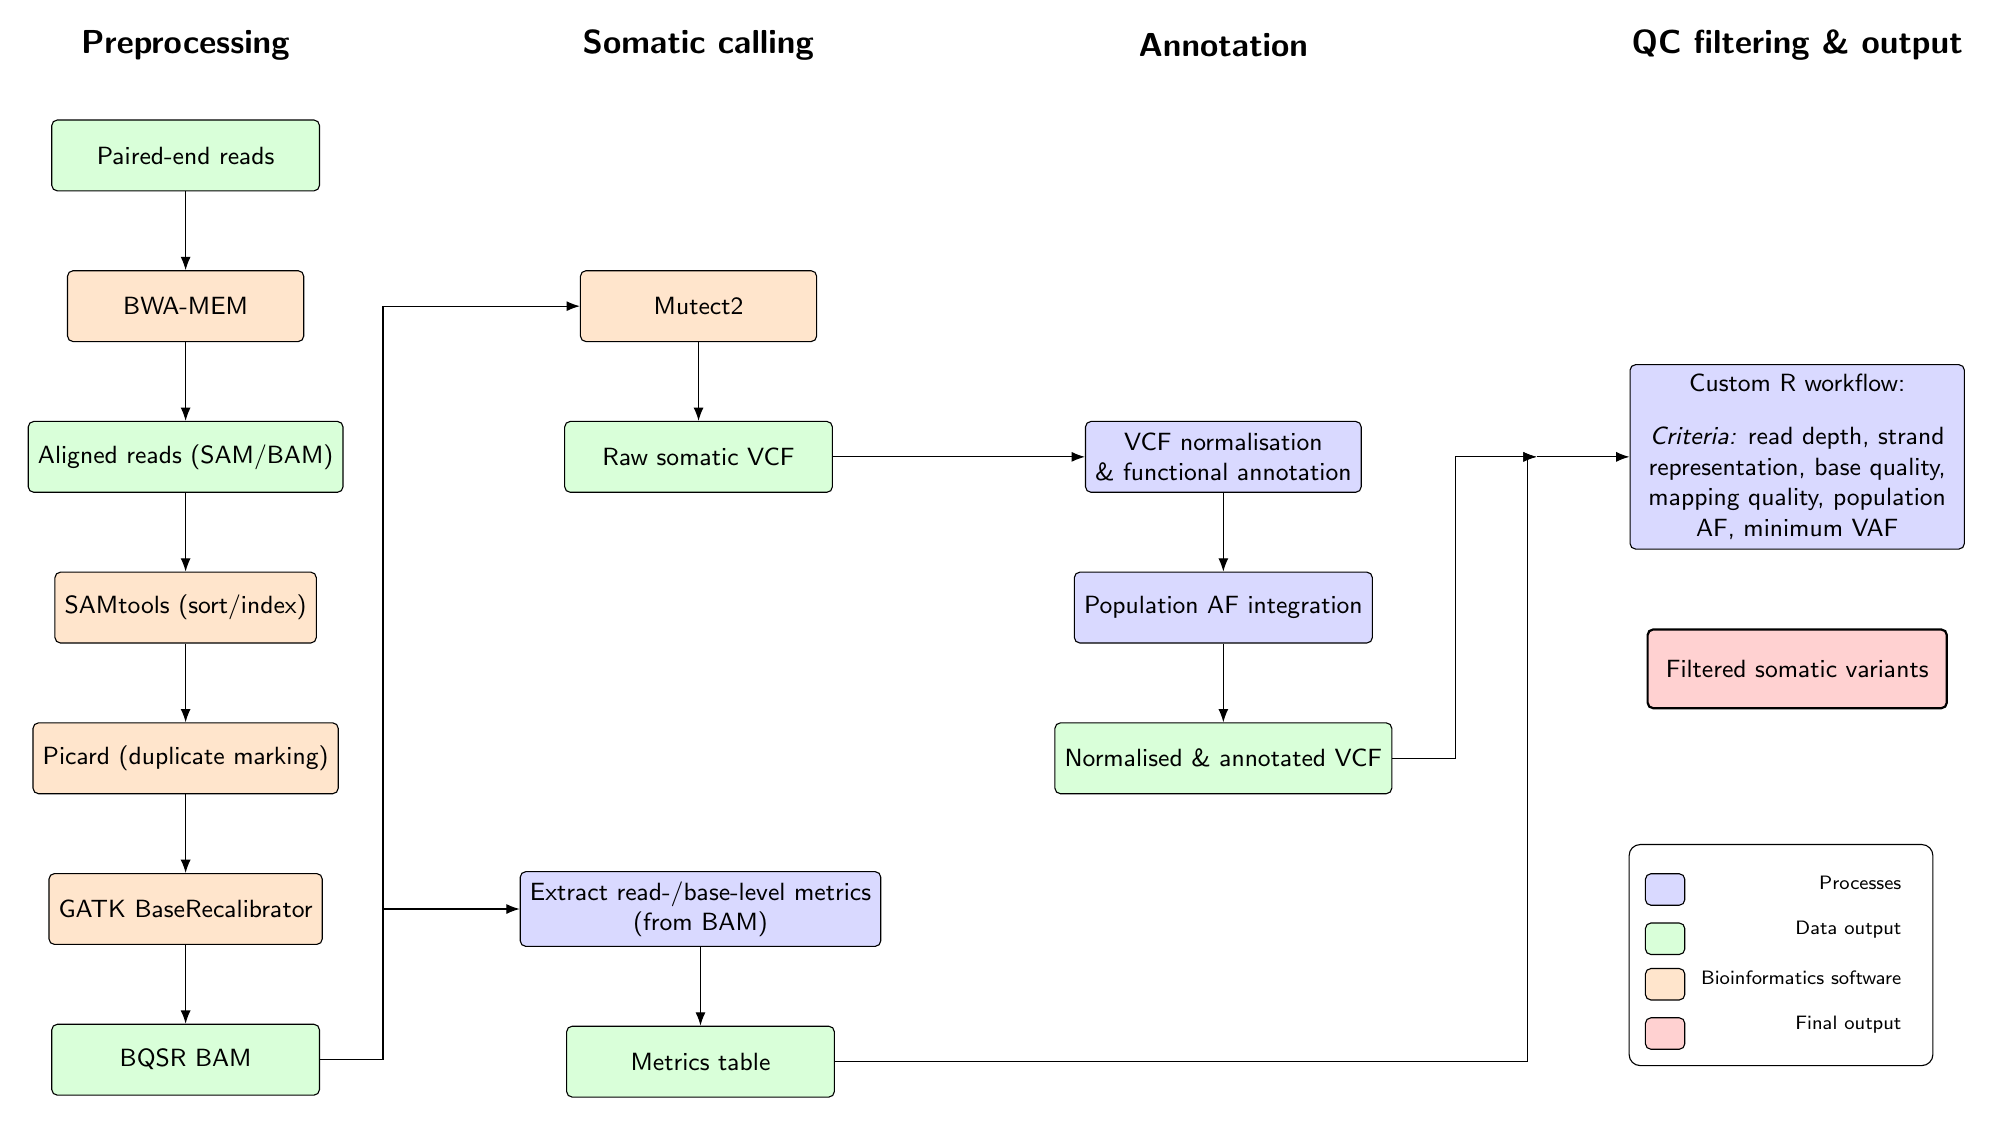
\begin{tikzpicture}[
		node distance=10mm and 16mm,
		>=Latex,
		font=\sffamily\small,
		process/.style  ={draw, rounded corners=2pt, fill=blue!15,  align=center, inner sep=3.5pt, minimum width=28mm, minimum height=9mm},
		data/.style     ={draw, rounded corners=2pt, fill=green!15, align=center, inner sep=3.5pt, minimum width=34mm, minimum height=9mm},
		software/.style ={draw, rounded corners=2pt, fill=orange!20,align=center, inner sep=3.5pt, minimum width=30mm, minimum height=9mm},
		final/.style    ={draw, rounded corners=2pt, fill=red!18,   align=center, inner sep=4pt,  thick, minimum width=38mm, minimum height=10mm},
		thinarrow/.style={->, line width=0.4pt},
		lab/.style={align=left, font=\sffamily\large, inner sep=1pt}
		]
		
		% --- Lane titles ---
%		\node[lab] (lane1) at (0,1.2) {\textbf{Preprocessing}};
%		\node[lab] (lane2) at (6.5,1.2) {\textbf{Somatic calling}};
%		\node[lab] (lane3) at (12.8,1.2) {\textbf{Annotation}};
%		\node[lab] (lane5) at (20.0,1.2) {\textbf{QC filtering \& output}};
		
		% --- Column 1: Preprocessing ---
		\node[data]     (paired)                        {Paired-end reads};
		\node[software, below=of paired] (bwa)         {BWA-MEM};
		\node[data,     below=of bwa]    (aligned)     {Aligned reads (SAM/BAM)};
		\node[software, below=of aligned](samtools)    {SAMtools (sort/index)};
		\node[software, below=of samtools](picard)     {Picard (duplicate marking)};
		\node[software, below=of picard] (bqsr)        {GATK BaseRecalibrator};
		\node[data,     below=of bqsr]   (recal)       {BQSR BAM};
		
		\draw[thinarrow] (paired)   -- (bwa);
		\draw[thinarrow] (bwa)      -- (aligned);
		\draw[thinarrow] (aligned)  -- (samtools);
		\draw[thinarrow] (samtools) -- (picard);
		\draw[thinarrow] (picard)   -- (bqsr);
		\draw[thinarrow] (bqsr)     -- (recal);
		
		% --- Column 2: Somatic calling ---
		\node[software, right=35mm of bwa]   (mutect)  {Mutect2};
		\node[data,     below=of mutect]     (rawvcf)  {Raw somatic VCF};
		
		\draw[thinarrow] (recal.east) -- ++(8mm,0) |- (mutect);
		\draw[thinarrow] (mutect)     -- (rawvcf);

		% --- Column 2: Metric extraction  ---
		\node[process,  right=25mm of bqsr, yshift=0mm] (metrics) {Extract read-/base-level metrics \\ (from BAM)};
		\node[data,     below=of metrics] (mettab) {Metrics table};
		
		% elbow route: right – up – right from BQSR BAM to metrics
		\draw[thinarrow] (recal.east) -- ++(8mm,0) |- (metrics.west);
		\draw[thinarrow] (metrics) -- (mettab);
		
		% --- Column 3: Normalisation & functional annotation ---
		\node[process,  right=32mm of rawvcf] (normann) {VCF normalisation \\ \& functional annotation};
		\node[process,  below=of normann]     (afint)   {Population AF integration};
		\node[data,     below=of afint]       (annvcf)  {Normalised \& annotated VCF};
		
		\draw[thinarrow] (rawvcf.east) -- (normann.west);
		\draw[thinarrow] (normann)     -- (afint);
		\draw[thinarrow] (afint)       -- (annvcf);
		
	
		% --- Column 5: R-based filtering and final output ---
		\node[process,  right=34mm of normann] (rfilt) {Custom R workflow:\\ \\[1pt]
			\begin{minipage}{40mm}\centering
				\textit{Criteria:} read depth, strand representation, base quality, mapping quality, population AF, minimum VAF
		\end{minipage}};
		\node[final,    below=of rfilt]        (finalout) {Filtered somatic variants};
		
		% Route around the annotation box
		%\draw[thinarrow] (annvcf.east) -- ++(8mm,0) |- (rfilt.west);
		%\draw[thinarrow] (mettab.east) -- ++(88mm,0) |- (rfilt.west);
		%\draw[thinarrow] (rfilt) -- (finalout);
		
		
		% --- Merge both inputs with visible arrowheads at the junction ---
		\coordinate (rfilt_in) at (rfilt.west);
		\coordinate (join)     at ($(rfilt_in)+(-11.8mm,0)$);
		  % adjust offset if needed
		
		\draw[thinarrow] (annvcf.east) -- ++(8mm,0) |- (join);          % arrowhead at join
		\draw[thinarrow] (mettab.east) -- ++(88mm,0) |- (join);          % arrowhead at join
		\draw[thinarrow] (join) -- (rfilt_in);                          % final short segment
		
		% --- Compact colour key in bottom-right (outside the flow) ---
		\matrix[anchor=south east, draw, rounded corners, inner sep=2mm, fill=white]
		(legend) at ($(current bounding box.south east)+(-4mm,4mm)$)
		{
			\node[draw, rounded corners=2pt, fill=blue!15,  minimum width=5mm, minimum height=4mm] {}; & \node{\scriptsize Processes}; \\
			\node[draw, rounded corners=2pt, fill=green!15, minimum width=5mm, minimum height=4mm] {}; & \node{\scriptsize Data output}; \\
			\node[draw, rounded corners=2pt, fill=orange!20,minimum width=5mm, minimum height=4mm] {}; & \node{\scriptsize Bioinformatics software}; \\
			\node[draw, rounded corners=2pt, fill=red!18,   minimum width=5mm, minimum height=4mm] {}; & \node{\scriptsize Final output}; \\
		};

		% Create a common horizontal baseline slightly above the top row
		\coordinate (titleline) at (0,1.4); % adjust 1.4 up/down for spacing
		
		\node[lab] at ($(paired |- titleline)$) {\textbf{Preprocessing}};
		\node[lab] at ($(mutect |- titleline)$) {\textbf{Somatic calling}};
		\node[lab] at ($(normann |- titleline)$) {\textbf{Annotation}};
		\node[lab] at ($(rfilt |- titleline)$) {\textbf{QC filtering \& output}};
		
	\end{tikzpicture}
\end{document}
